%%%%%%%%%%%%%%%%%%%%%%%%%%%%%%%%%%%%%%%%%%%%%%%%%%%
%% P3: Phenomenology of Particle Physics                         
%%
%% Author:  André Rubbia                   		 
%%
%% Figure 29.12 Fit of the Higgs boson mass within the SM computed with GFITTER.
%%
%% This work is licensed under the Creative Commons Attribution 4.0 International License. 
%% To view a copy of this license, visit http://creativecommons.org/licenses/by/4.0/ or 
%% send a letter to Creative Commons, PO Box 1866, Mountain View, CA 94042, USA.
%%
%%%%%%%%%%%%%%%%%%%%%%%%%%%%%%%%%%%%%%%%%%%%%%%%%%%

\documentclass[a4paper,10pt]{article}

\usepackage[T1]{fontenc}
\usepackage[utf8]{inputenc}
\usepackage{lmodern}
\usepackage[labelfont=bf]{caption}
\usepackage{upgreek}

\usepackage{tikz}
\usepackage{pgfplots}
\pgfplotsset{compat=1.17}
\usepgfplotslibrary{ternary}
\usepgfplotslibrary{fillbetween}
\usepgfplotslibrary{external}

\def\d{\mathrm{d}}
\setlength{\oddsidemargin}{-1.0cm}
\setlength{\evensidemargin}{-1.0cm}
\setlength{\textheight}{25cm}
\setlength{\textwidth}{18cm}

\pgfkeys{/pgf/number format/.cd,1000 sep={}}

\begin{document}

%%%%%%%%%%%%%%%%   FIGURE  %%%%%%%%%%%%%%%%%%%%%%%%%%%%%%
\begin{figure}[htb]
\centering
\begin{tikzpicture}[scale=1.]
\begin{axis}[xmin=0, xmax=250,
	ymin=0, ymax=9, ytick={0,1,4,9},
	title=Standard Model Fit (GFITTERv2.2),
	xlabel=$m_H$ (GeV),
	ylabel=$\Delta \chi^2$,
	xmajorgrids=true,
	ymajorgrids=true,
	]

    \addplot[very thick,
    color=blue,
    no marks,
    ] coordinates {
(    21.9,  12.92)
(    25.7,  10.78)
(    29.5,  8.969)
(    33.3,  7.422)
(    37.1,    6.1)
(    40.9,  4.969)
(    44.7,  4.002)
(    48.5,  3.179)
(    52.3,  2.481)
(    56.1,  1.893)
(    59.9,  1.404)
(    63.7,  1.002)
(    67.5, 0.6789)
(    71.3, 0.4264)
(    75.1,  0.238)
(    78.9, 0.1075)
(    82.7,0.02991)
(    86.5,0.0005095)
(    90.3,0.01525)
(    94.1,0.07049)
(    97.9,  0.163)
(   101.7, 0.2898)
(   105.5, 0.4483)
(   109.3, 0.6361)
(   113.1, 0.8511)
(   116.9,  1.091)
(   120.7,  1.355)
(   124.5,   1.64)
(   128.3,  1.946)
(   132.1,   2.27)
(   135.9,  2.612)
(   139.7,  2.971)
(   143.5,  3.345)
(   147.3,  3.734)
(   151.1,  4.136)
(   154.9,   4.55)
(   158.7,  4.977)
(   162.5,  5.414)
(   166.3,  5.862)
(   170.1,   6.32)
(   173.9,  6.787)
(   177.7,  7.263)
(   181.5,  7.746)
(   185.3,  8.237)
(   189.1,  8.736)
(   192.9,  9.241)
(   196.7,  9.752)
(   200.5,  10.27)
};

\end{axis}
\end{tikzpicture}
	\caption{Fit of the Higgs boson mass within the SM computed with GFITTER.}
\end{figure}
%
%%%%%%%%%%%%%%%%   END FIGURE  %%%%%%%%%%%%%%%%%%%%%%%%%%%%%%
%


\end{document}
